% Options for packages loaded elsewhere
\PassOptionsToPackage{unicode}{hyperref}
\PassOptionsToPackage{hyphens}{url}
%
\documentclass[
  ignorenonframetext,
]{beamer}
\usepackage{pgfpages}
\setbeamertemplate{caption}[numbered]
\setbeamertemplate{caption label separator}{: }
\setbeamercolor{caption name}{fg=normal text.fg}
\beamertemplatenavigationsymbolsempty
% Prevent slide breaks in the middle of a paragraph
\widowpenalties 1 10000
\raggedbottom
\setbeamertemplate{part page}{
  \centering
  \begin{beamercolorbox}[sep=16pt,center]{part title}
    \usebeamerfont{part title}\insertpart\par
  \end{beamercolorbox}
}
\setbeamertemplate{section page}{
  \centering
  \begin{beamercolorbox}[sep=12pt,center]{part title}
    \usebeamerfont{section title}\insertsection\par
  \end{beamercolorbox}
}
\setbeamertemplate{subsection page}{
  \centering
  \begin{beamercolorbox}[sep=8pt,center]{part title}
    \usebeamerfont{subsection title}\insertsubsection\par
  \end{beamercolorbox}
}
\AtBeginPart{
  \frame{\partpage}
}
\AtBeginSection{
  \ifbibliography
  \else
    \frame{\sectionpage}
  \fi
}
\AtBeginSubsection{
  \frame{\subsectionpage}
}
\usepackage{lmodern}
\usepackage{amsmath}
\usepackage{ifxetex,ifluatex}
\ifnum 0\ifxetex 1\fi\ifluatex 1\fi=0 % if pdftex
  \usepackage[T1]{fontenc}
  \usepackage[utf8]{inputenc}
  \usepackage{textcomp} % provide euro and other symbols
  \usepackage{amssymb}
\else % if luatex or xetex
  \usepackage{unicode-math}
  \defaultfontfeatures{Scale=MatchLowercase}
  \defaultfontfeatures[\rmfamily]{Ligatures=TeX,Scale=1}
\fi
\usetheme[]{Boadilla}
\usecolortheme{beaver}
% Use upquote if available, for straight quotes in verbatim environments
\IfFileExists{upquote.sty}{\usepackage{upquote}}{}
\IfFileExists{microtype.sty}{% use microtype if available
  \usepackage[]{microtype}
  \UseMicrotypeSet[protrusion]{basicmath} % disable protrusion for tt fonts
}{}
\makeatletter
\@ifundefined{KOMAClassName}{% if non-KOMA class
  \IfFileExists{parskip.sty}{%
    \usepackage{parskip}
  }{% else
    \setlength{\parindent}{0pt}
    \setlength{\parskip}{6pt plus 2pt minus 1pt}}
}{% if KOMA class
  \KOMAoptions{parskip=half}}
\makeatother
\usepackage{xcolor}
\IfFileExists{xurl.sty}{\usepackage{xurl}}{} % add URL line breaks if available
\IfFileExists{bookmark.sty}{\usepackage{bookmark}}{\usepackage{hyperref}}
\hypersetup{
  pdftitle={MATH513 Practical Presentation},
  pdfauthor={10570155, 10696253, 10701983},
  hidelinks,
  pdfcreator={LaTeX via pandoc}}
\urlstyle{same} % disable monospaced font for URLs
\newif\ifbibliography
\usepackage{color}
\usepackage{fancyvrb}
\newcommand{\VerbBar}{|}
\newcommand{\VERB}{\Verb[commandchars=\\\{\}]}
\DefineVerbatimEnvironment{Highlighting}{Verbatim}{commandchars=\\\{\}}
% Add ',fontsize=\small' for more characters per line
\usepackage{framed}
\definecolor{shadecolor}{RGB}{248,248,248}
\newenvironment{Shaded}{\begin{snugshade}}{\end{snugshade}}
\newcommand{\AlertTok}[1]{\textcolor[rgb]{0.94,0.16,0.16}{#1}}
\newcommand{\AnnotationTok}[1]{\textcolor[rgb]{0.56,0.35,0.01}{\textbf{\textit{#1}}}}
\newcommand{\AttributeTok}[1]{\textcolor[rgb]{0.77,0.63,0.00}{#1}}
\newcommand{\BaseNTok}[1]{\textcolor[rgb]{0.00,0.00,0.81}{#1}}
\newcommand{\BuiltInTok}[1]{#1}
\newcommand{\CharTok}[1]{\textcolor[rgb]{0.31,0.60,0.02}{#1}}
\newcommand{\CommentTok}[1]{\textcolor[rgb]{0.56,0.35,0.01}{\textit{#1}}}
\newcommand{\CommentVarTok}[1]{\textcolor[rgb]{0.56,0.35,0.01}{\textbf{\textit{#1}}}}
\newcommand{\ConstantTok}[1]{\textcolor[rgb]{0.00,0.00,0.00}{#1}}
\newcommand{\ControlFlowTok}[1]{\textcolor[rgb]{0.13,0.29,0.53}{\textbf{#1}}}
\newcommand{\DataTypeTok}[1]{\textcolor[rgb]{0.13,0.29,0.53}{#1}}
\newcommand{\DecValTok}[1]{\textcolor[rgb]{0.00,0.00,0.81}{#1}}
\newcommand{\DocumentationTok}[1]{\textcolor[rgb]{0.56,0.35,0.01}{\textbf{\textit{#1}}}}
\newcommand{\ErrorTok}[1]{\textcolor[rgb]{0.64,0.00,0.00}{\textbf{#1}}}
\newcommand{\ExtensionTok}[1]{#1}
\newcommand{\FloatTok}[1]{\textcolor[rgb]{0.00,0.00,0.81}{#1}}
\newcommand{\FunctionTok}[1]{\textcolor[rgb]{0.00,0.00,0.00}{#1}}
\newcommand{\ImportTok}[1]{#1}
\newcommand{\InformationTok}[1]{\textcolor[rgb]{0.56,0.35,0.01}{\textbf{\textit{#1}}}}
\newcommand{\KeywordTok}[1]{\textcolor[rgb]{0.13,0.29,0.53}{\textbf{#1}}}
\newcommand{\NormalTok}[1]{#1}
\newcommand{\OperatorTok}[1]{\textcolor[rgb]{0.81,0.36,0.00}{\textbf{#1}}}
\newcommand{\OtherTok}[1]{\textcolor[rgb]{0.56,0.35,0.01}{#1}}
\newcommand{\PreprocessorTok}[1]{\textcolor[rgb]{0.56,0.35,0.01}{\textit{#1}}}
\newcommand{\RegionMarkerTok}[1]{#1}
\newcommand{\SpecialCharTok}[1]{\textcolor[rgb]{0.00,0.00,0.00}{#1}}
\newcommand{\SpecialStringTok}[1]{\textcolor[rgb]{0.31,0.60,0.02}{#1}}
\newcommand{\StringTok}[1]{\textcolor[rgb]{0.31,0.60,0.02}{#1}}
\newcommand{\VariableTok}[1]{\textcolor[rgb]{0.00,0.00,0.00}{#1}}
\newcommand{\VerbatimStringTok}[1]{\textcolor[rgb]{0.31,0.60,0.02}{#1}}
\newcommand{\WarningTok}[1]{\textcolor[rgb]{0.56,0.35,0.01}{\textbf{\textit{#1}}}}
\usepackage{longtable,booktabs}
\usepackage{calc} % for calculating minipage widths
\usepackage{caption}
% Make caption package work with longtable
\makeatletter
\def\fnum@table{\tablename~\thetable}
\makeatother
\usepackage{graphicx}
\makeatletter
\def\maxwidth{\ifdim\Gin@nat@width>\linewidth\linewidth\else\Gin@nat@width\fi}
\def\maxheight{\ifdim\Gin@nat@height>\textheight\textheight\else\Gin@nat@height\fi}
\makeatother
% Scale images if necessary, so that they will not overflow the page
% margins by default, and it is still possible to overwrite the defaults
% using explicit options in \includegraphics[width, height, ...]{}
\setkeys{Gin}{width=\maxwidth,height=\maxheight,keepaspectratio}
% Set default figure placement to htbp
\makeatletter
\def\fps@figure{htbp}
\makeatother
\setlength{\emergencystretch}{3em} % prevent overfull lines
\providecommand{\tightlist}{%
  \setlength{\itemsep}{0pt}\setlength{\parskip}{0pt}}
\setcounter{secnumdepth}{-\maxdimen} % remove section numbering
\ifluatex
  \usepackage{selnolig}  % disable illegal ligatures
\fi

\title{MATH513 Practical Presentation}
\author{10570155, 10696253, 10701983}
\date{10/12/2020}

\begin{document}
\frame{\titlepage}

\begin{frame}{Introduction}
\protect\hypertarget{introduction}{}
\begin{itemize}
\tightlist
\item
  Samsung and Apple
\item
  Flagship phones chosen

  \begin{itemize}
  \tightlist
  \item
    S20FE
  \item
    iPhone12
  \item
    S20
  \end{itemize}
\end{itemize}

\textbf{Tools Utilised}

\begin{itemize}
\tightlist
\item
  Rstudio
\item
  RTweet
\item
  Twitter Developer API
\item
  GitHub
\end{itemize}

\begin{figure}

{\centering 
\includegraphics[width=0.15\linewidth]{./Images/Logos/apple_logo} 
\includegraphics[width=0.15\linewidth]{./Images/Logos/samsung_logo} 
\includegraphics[width=0.15\linewidth]{./Images/Logos/rstudio_logo} 
\includegraphics[width=0.15\linewidth]{./Images/Logos/twitter_logo} 

}

\end{figure}
\end{frame}

\begin{frame}{Research}
\protect\hypertarget{research}{}
\textbf{Choosing Twitter for Analysis}

\begin{itemize}
\tightlist
\item
  Open API Access compared to others
\item
  Almost all data is public
\item
  Advanced filtering and queries
\item
  Generous Rate limiting
\end{itemize}

\textbf{Hashtags}

\begin{itemize}
\tightlist
\item
  @SamsungMobile - \url{https://twitter.com/SamsungMobile}
\item
  @Apple - \url{https://twitter.com/Apple}
\item
  @tim\_cook - \url{https://twitter.com/tim_cook}
\end{itemize}
\end{frame}

\begin{frame}{Data Cleaning and Feature Engineering}
\protect\hypertarget{data-cleaning-and-feature-engineering}{}
\textbf{Data Cleaning}

\begin{itemize}
\tightlist
\item
  Duplicate tweet and user observations were removed
\item
  Tweet text and user bios were cleaned

  \begin{itemize}
  \tightlist
  \item
    Removed links, hash-tags, emojis, and user mentions
  \end{itemize}
\end{itemize}

\textbf{Feature Engineering}

\begin{itemize}
\tightlist
\item
  Users were marked as potential bots
\item
  User country was extracted from the location of their profile
\item
  Tweets were marked as potential spam
\item
  Hash-tags were extracted from the tweet text
\item
  Product features were extracted from the tweet text

  \begin{itemize}
  \tightlist
  \item
    Display, Battery, Camera, Price, and 5G Capability
  \end{itemize}
\item
  An overall sentiment score was calculated for each tweet
\end{itemize}
\end{frame}

\begin{frame}[fragile]{Summary of Collected Data}
\protect\hypertarget{summary-of-collected-data}{}
\textbf{Total Tweets:} 73690 after data cleaning

\textbf{Total Features:}
\texttt{5\ (Display,\ Battery,\ Camera,\ Price,\ and\ 5G)}

\begin{longtable}[]{@{}lrll@{}}
\caption{Summary of Tweet Data}\tabularnewline
\toprule
Product & Number of Tweets & \% Spam Tweets & \% Feature
Tweets\tabularnewline
\midrule
\endfirsthead
\toprule
Product & Number of Tweets & \% Spam Tweets & \% Feature
Tweets\tabularnewline
\midrule
\endhead
Galaxy S20 & 13147 & 3\% & 20\%\tabularnewline
Galaxy S20 FE & 28923 & 19\% & 19\%\tabularnewline
iPhone12 & 31620 & 13\% & 7\%\tabularnewline
\bottomrule
\end{longtable}

\begin{longtable}[]{@{}rlr@{}}
\caption{Summary of User Data}\tabularnewline
\toprule
Number of Users & \% Bot Users & Unique Countries\tabularnewline
\midrule
\endfirsthead
\toprule
Number of Users & \% Bot Users & Unique Countries\tabularnewline
\midrule
\endhead
35051 & \textgreater1\% & 163\tabularnewline
\bottomrule
\end{longtable}
\end{frame}

\begin{frame}{Time Periods for Data Collection}
\protect\hypertarget{time-periods-for-data-collection}{}
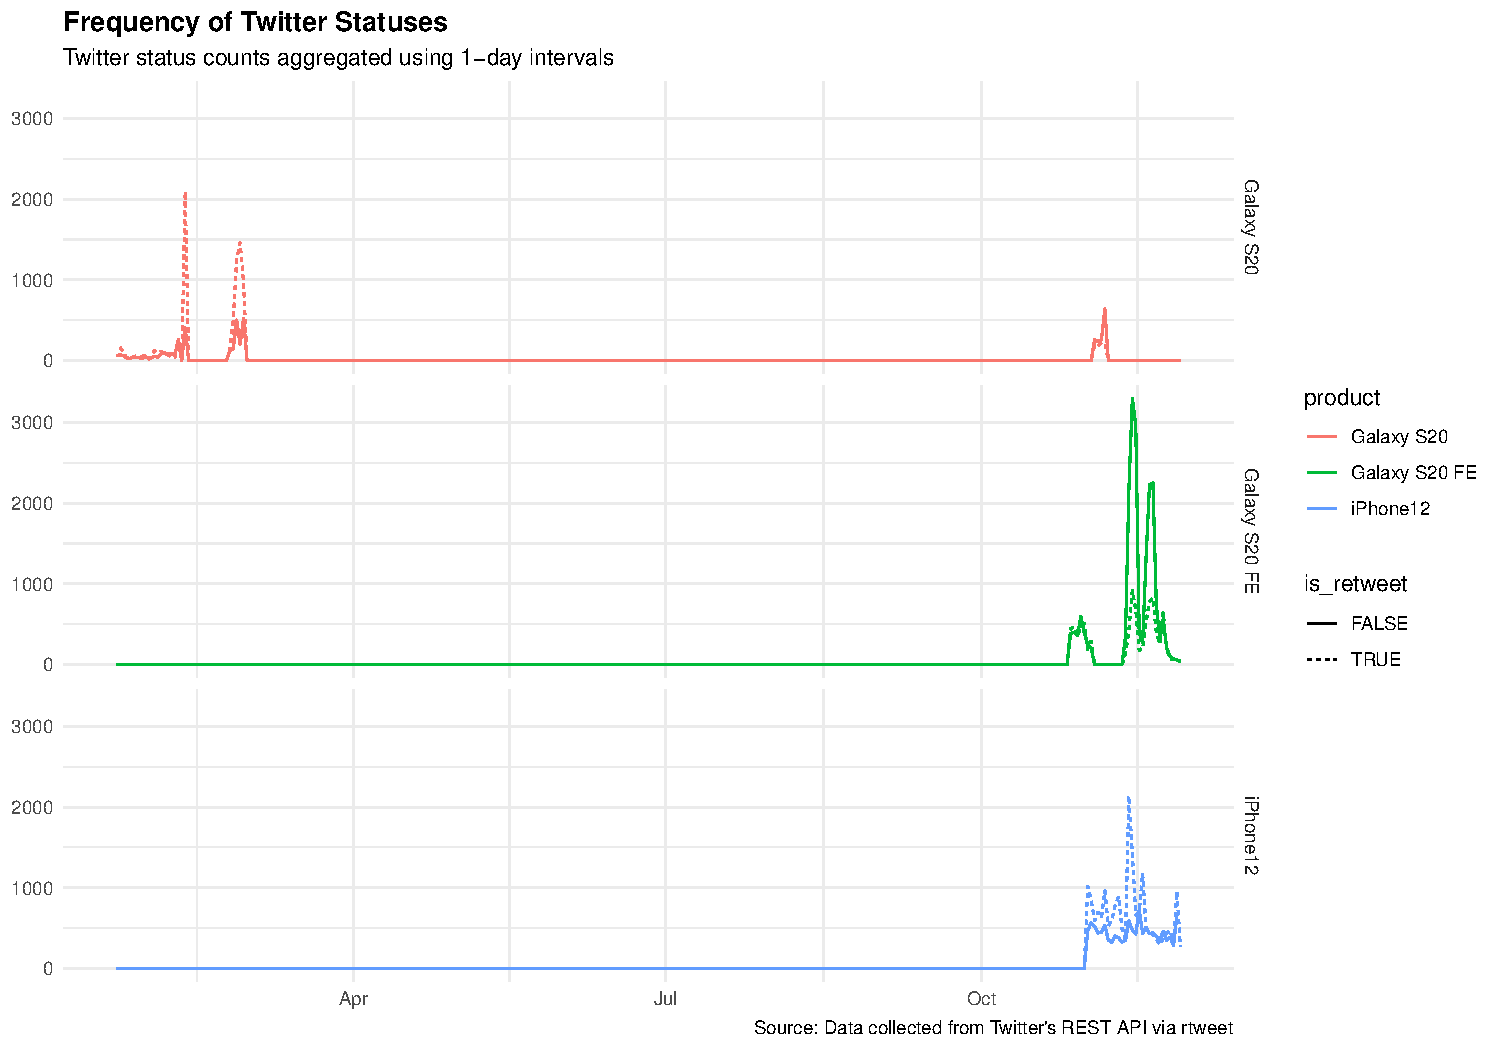
\includegraphics{SocialMedia_10570155_10696253_10701983_files/figure-beamer/unnamed-chunk-1-1.pdf}
\end{frame}

\begin{frame}{Results - Sentiment Analysis - All Tweets}
\protect\hypertarget{results---sentiment-analysis---all-tweets}{}
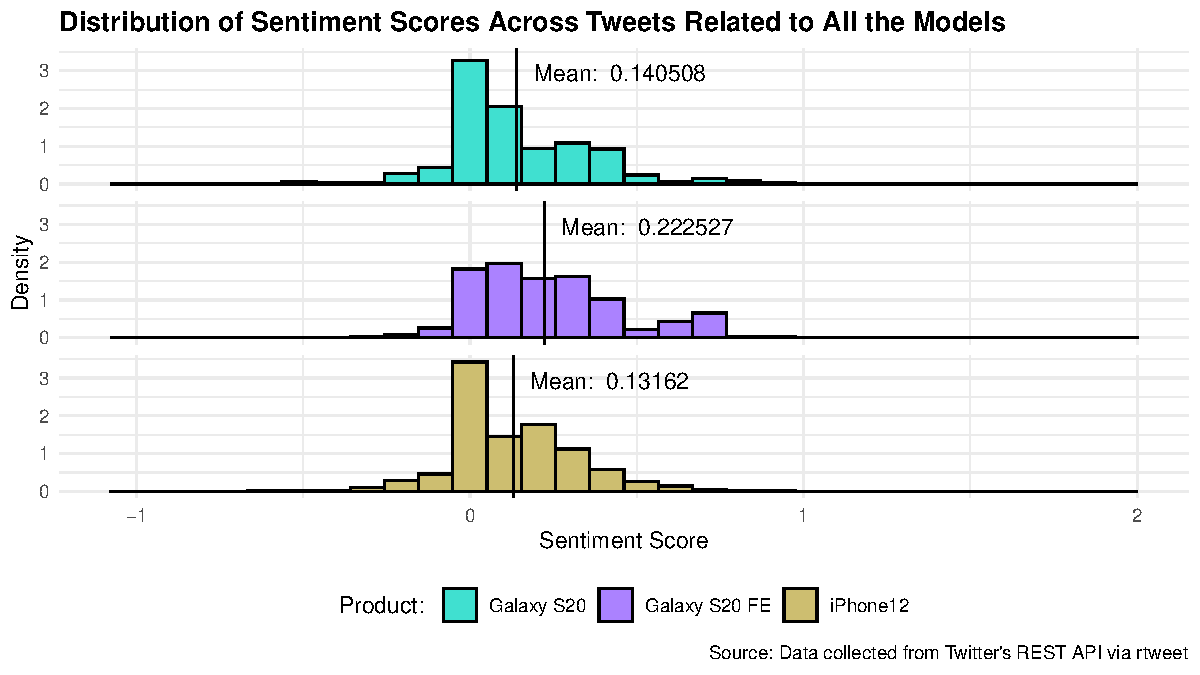
\includegraphics{SocialMedia_10570155_10696253_10701983_files/figure-beamer/unnamed-chunk-3-1.pdf}
\end{frame}

\begin{frame}{Results - Sentiment Analysis - Features}
\protect\hypertarget{results---sentiment-analysis---features}{}
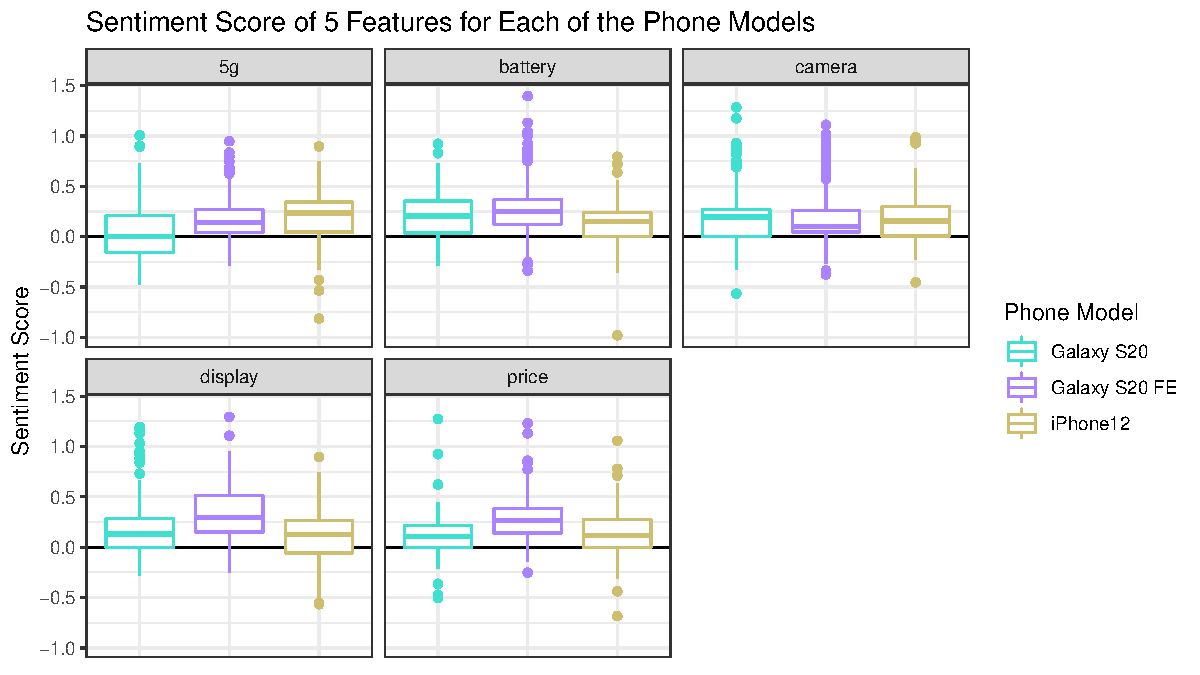
\includegraphics{SocialMedia_10570155_10696253_10701983_files/figure-beamer/unnamed-chunk-5-1.pdf}
\end{frame}

\begin{frame}{Results - Sentiment Globally}
\protect\hypertarget{results---sentiment-globally}{}
\begin{figure}

{\centering \includegraphics[width=0.4\linewidth]{SocialMedia_10570155_10696253_10701983_files/figure-beamer/unnamed-chunk-7-1} \includegraphics[width=0.4\linewidth]{SocialMedia_10570155_10696253_10701983_files/figure-beamer/unnamed-chunk-7-2} 

}

\end{figure}

\begin{center}\includegraphics[width=0.4\linewidth]{SocialMedia_10570155_10696253_10701983_files/figure-beamer/unnamed-chunk-8-1} \end{center}

!!!!! STOCK PRICE VS SENTIMENT
\end{frame}

\begin{frame}{Improvements \& Further Study}
\protect\hypertarget{improvements-further-study}{}
\textbf{Improvements}

Google Maps API to have region filter

Look at mentions of apple in samsung and vice versa
\end{frame}

\begin{frame}{Issues and overcoming them}
\protect\hypertarget{issues-and-overcoming-them}{}
\begin{itemize}
\tightlist
\item
  Extraction by date
\item
  Duplication
\item
  Time limits
\item
  Foreign languages
\item
\end{itemize}
\end{frame}

\begin{frame}{Conclusions}
\protect\hypertarget{conclusions}{}
\begin{itemize}
\item
  Twitter data provides up to date information for companies to analyse
  for customer feedback
\item
  Data can provide useful information to guide product teams when
  analysed correctly
\end{itemize}
\end{frame}

\begin{frame}{References}
\protect\hypertarget{references}{}
\begin{itemize}
\item
  Ahmed, Wasim (2019) \emph{Using Twitter as a data source: an overview
  of social media research tools} Available at:
  \url{https://blogs.lse.ac.uk/impactofsocialsciences/2019/06/18/using-twitter-as-a-data-source-an-overview-of-social-media-research-tools-2019/}
  (Accessed: 07 December 2020)
\item
  Dalla Valle, Luciana (2020) \emph{MATH513 Lecture and Tutorial Code}
  Available at:
  \url{https://dle.plymouth.ac.uk/course/view.php?id=49628} (Accessed:
  2020)
\item
  Fuchs, Matti (2018) \emph{Doing your first sentiment analysis in R
  with Sentimentr} Available at:
  \url{https://towardsdatascience.com/doing-your-first-sentiment-analysis-in-r-with-sentimentr-167855445132}
  (Accessed: 06 December 2020)
\item
  Rinker, Tyler (2020) \emph{R Documentation - sentiment\_by} Available
  at:
  \url{https://www.rdocumentation.org/packages/sentimentr/versions/2.7.1/topics/sentiment_by}
  (Accessed: 06 December 2020)
\item
  RStudio (2020) \emph{R Markdown Cheat Sheet} Available at:
  \url{https://www.rstudio.com/wp-content/uploads/2015/02/rmarkdown-cheatsheet.pdf}
  (Accessed: 10 October 2020)
\item
  RStudio (2014) \emph{R Markdown Reference Guide} Available at:
  \url{https://www.rstudio.com/wp-content/uploads/2015/03/rmarkdown-reference.pdf}
  (Accessed: 10 October 2020)
\end{itemize}
\end{frame}

\begin{frame}[fragile]{References}
\protect\hypertarget{references-1}{}
\begin{itemize}
\item
  Twitter (2020) \emph{API Documentation} Available at:
  \url{https://developer.twitter.com/en/docs/twitter-api} (Accessed: 10
  October 2020)
\item
  Young, Michelle (2017) \emph{Twitter Data Mining: A Guide to Big Data
  Analytics Using Python} Available at:
  \url{https://chatbotslife.com/twitter-data-mining-a-guide-to-big-data-analytics-using-python-4efc8ccfa219}
  (Accessed: 07 December 2020)
\end{itemize}

\begin{Shaded}
\begin{Highlighting}[]
\FunctionTok{citation}\NormalTok{()}
\end{Highlighting}
\end{Shaded}

\begin{verbatim}
## 
## To cite R in publications use:
## 
##   R Core Team (2020). R: A language and environment for statistical
##   computing. R Foundation for Statistical Computing, Vienna, Austria.
##   URL https://www.R-project.org/.
## 
## A BibTeX entry for LaTeX users is
## 
##   @Manual{,
##     title = {R: A Language and Environment for Statistical Computing},
##     author = {{R Core Team}},
##     organization = {R Foundation for Statistical Computing},
##     address = {Vienna, Austria},
##     year = {2020},
##     url = {https://www.R-project.org/},
##   }
## 
## We have invested a lot of time and effort in creating R, please cite it
## when using it for data analysis. See also 'citation("pkgname")' for
## citing R packages.
\end{verbatim}
\end{frame}

\end{document}
